\subsubsection{Recirculation algorithm}
\label{sec:models-recirc} 

The \emph{Recirculation algorithm} designed by~\citet{hinton1988learning} is an unsupervised neural letwork for learning encoder tasks. Motivation for such a model comes from interesting hidden representations of backpropagation~(\ref{sec:models-bp}) with possible usage as an encoder. It has only two layers denoted \emph{visible layer} and \emph{hidden layer} as shown on figure~\ref{fig:models-recirc}. The aim of the network is to remember on the hidden layer the patterns presented to the visible layer. This could be used for compression if the hidden layer has fewer units than the visible layer. It also could be used as a content-addressable memory where if novel patterns are presented to the network it could show the most similar stored pattern. 

\begin{figure}[H]
  \centering
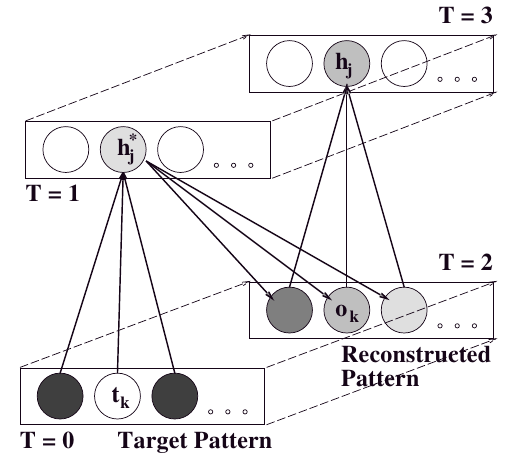
\includegraphics[width=0.4\textwidth]{img/recirculation.png}
  \caption{The recirculation algorithm by~\citet{hinton1988learning}. Taken from \citep{o1996bio}.}
  \label{fig:models-recirc}
\end{figure}

As depicted on figure~\ref{fig:models-recirc} activation is propagated in four steps $T \in \{0,1,2,3\}$. At the first phase denoted by $T=0$ only the input vector $t$ is clamped on the visible layer, at $T=1$ a forward pass $h^{*}$ is computed from visible to hidden, at $T=2$ a reconstructed pattern $o_k$ as a function of hidden state $h^{*}$ at $T=1$ is computed and finally at $T=3$ a hidden state $h$ is computed from $o_k$.

For the reconstruction to work \emph{symmetric} weights are used. The learning rule is common for both visible and hidden layers and it;s based only on difference of activations: 
\begin{align}
\frac{\partial E}{\partial w_{ij}} &= -(\eta^{*}_j - \eta_j) \phi'(\eta_j) t_k \nonumber \\
&\approx -(h^{*}_j - h_j)t_k \nonumber 
\end{align} 
The approximation step could be made because $\phi'(\eta_j)$ has \emph{usually} the same sign as $(\eta^{*}_j - \eta_j) $~\citep{hinton1988learning, o1996bio}. The approximation works better if the difference of activations is smaller and therefore, the activation for the reconstructed pattern $o$  is made similar to target pattern $t$: 
\begin{equation}
o_k = \alpha t_k + (1-\alpha)f(\eta_k). 
\end{equation} 

